\documentclass{article}
\usepackage{ctex}
\usepackage{graphicx}
\usepackage{amsmath}
\usepackage{indentfirst}
\usepackage{titlesec}
\usepackage{setspace}
\usepackage{subfigure}
\usepackage{caption}
\usepackage{float}
\usepackage{booktabs}
\usepackage{geometry}
\usepackage{multirow}
\usepackage{hyperref}
\hypersetup{
	colorlinks=true,
	linkcolor=blue,
	filecolor=magenta,      
	urlcolor=cyan,
	pdftitle={Overleaf Example},
	pdfpagemode=FullScreen,
}
\geometry{left=1.2cm,right=1.2cm,top=2cm,bottom=2cm}
\title{\songti \zihao{2}\bfseries HW6FFT}
\titleformat*{\section}{\songti\zihao{4}\bfseries}
\titleformat*{\subsection}{\songti\zihao{5}\bfseries}
\renewcommand\thesection{\arabic{section}}
\author{王启骅 PB20020580}
\begin{document}
	\maketitle
\section{结果与讨论}
计算得到f1对于$n=2^4$变换如图1,2,对于$ n=2^7 $的情况如图3,4,5(这里计算结果向量图太长分为两张)。对f2变换得到如图6,7,8。由图可见当n的取值越大,所构建得到的曲线越光滑,相应的可以获得有关信号的更多更广频率范围内的信息,逆变换得到的图像也更加接近原函数的图像。同样可以见到,当信号存在噪声时,FFT可以明显将噪声振幅减小,保留原信号。对于取前$ 25\% $的频率进行IFFT重建得到的信号,明显比原信号更加光滑,可见可以用该方法丢弃高频系数达到去噪声的目的。
\begin{figure}[!h]
	
	\centering
	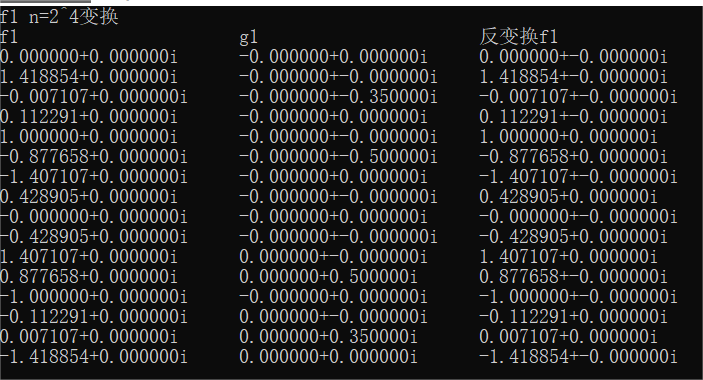
\includegraphics[scale=0.4]{f1}
	\captionsetup{font={small},labelfont=bf}
	\caption{\heiti\zihao{-5}f1进行FFT结果(n=$ 2^4 $)}
	\label{fig:1}
\end{figure}
	\begin{figure}[!h]
	
	\centering
	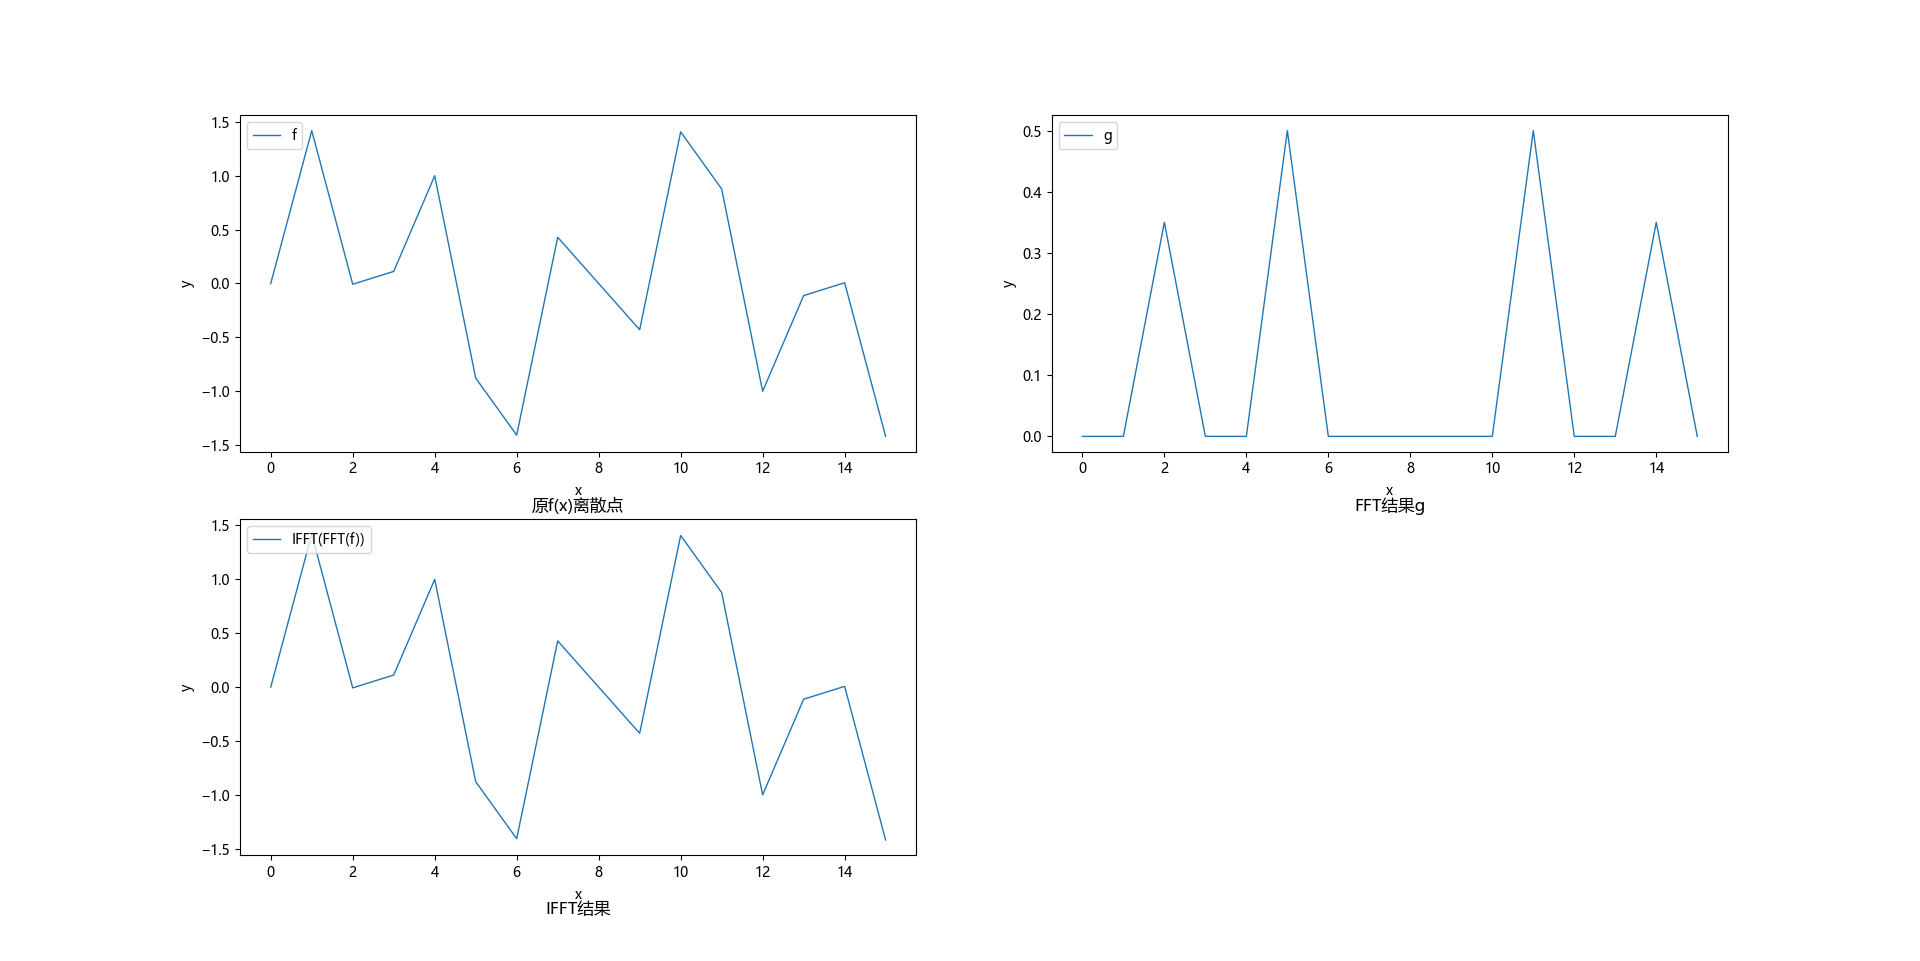
\includegraphics[scale=0.4]{f_1_4}
	\captionsetup{font={small},labelfont=bf}
	\caption{\heiti\zihao{-5}f1进行FFT结果(n=$ 2^4 $)}
	\label{fig:2}
\end{figure}
\begin{figure}[!h]
	
	\centering
	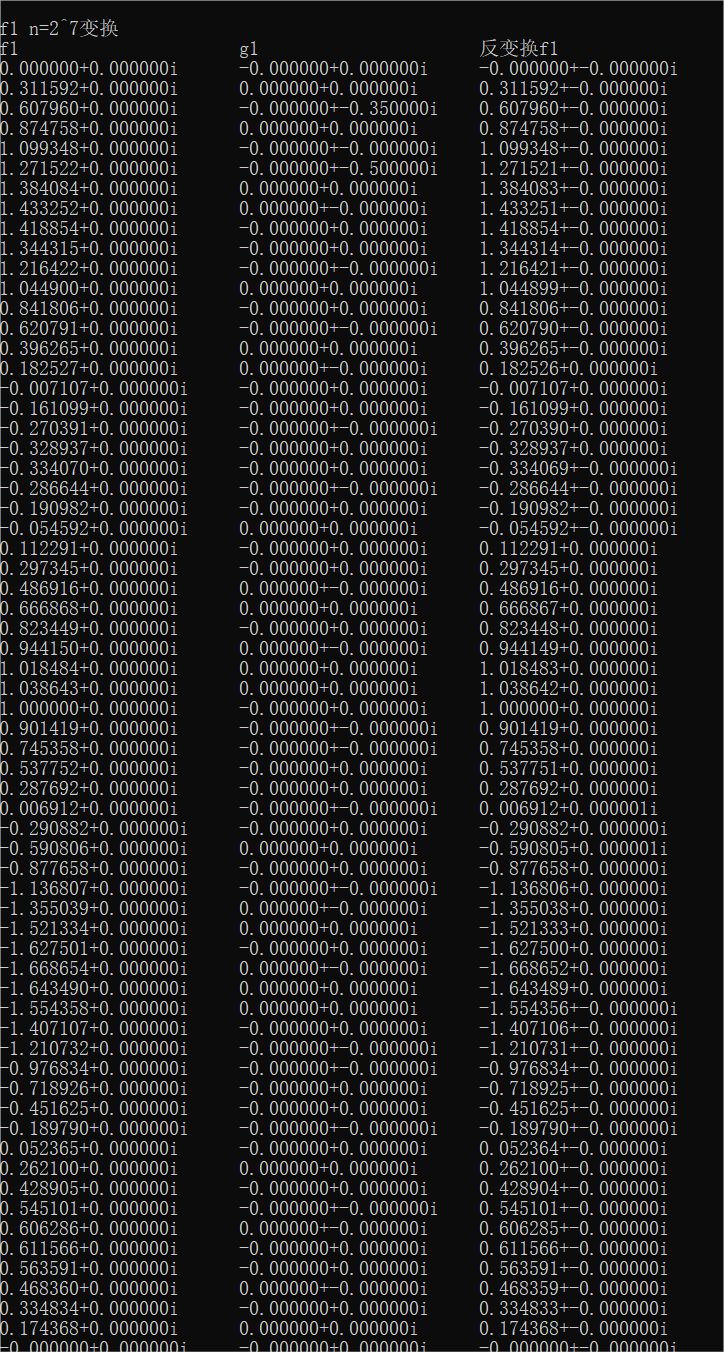
\includegraphics[scale=0.4]{f1_7(1)}
	\captionsetup{font={small},labelfont=bf}
	\caption{\heiti\zihao{-5}f1进行FFT结果(n=$ 2^7 $)1}

\end{figure}
\begin{figure}[!h]
	
	\centering
	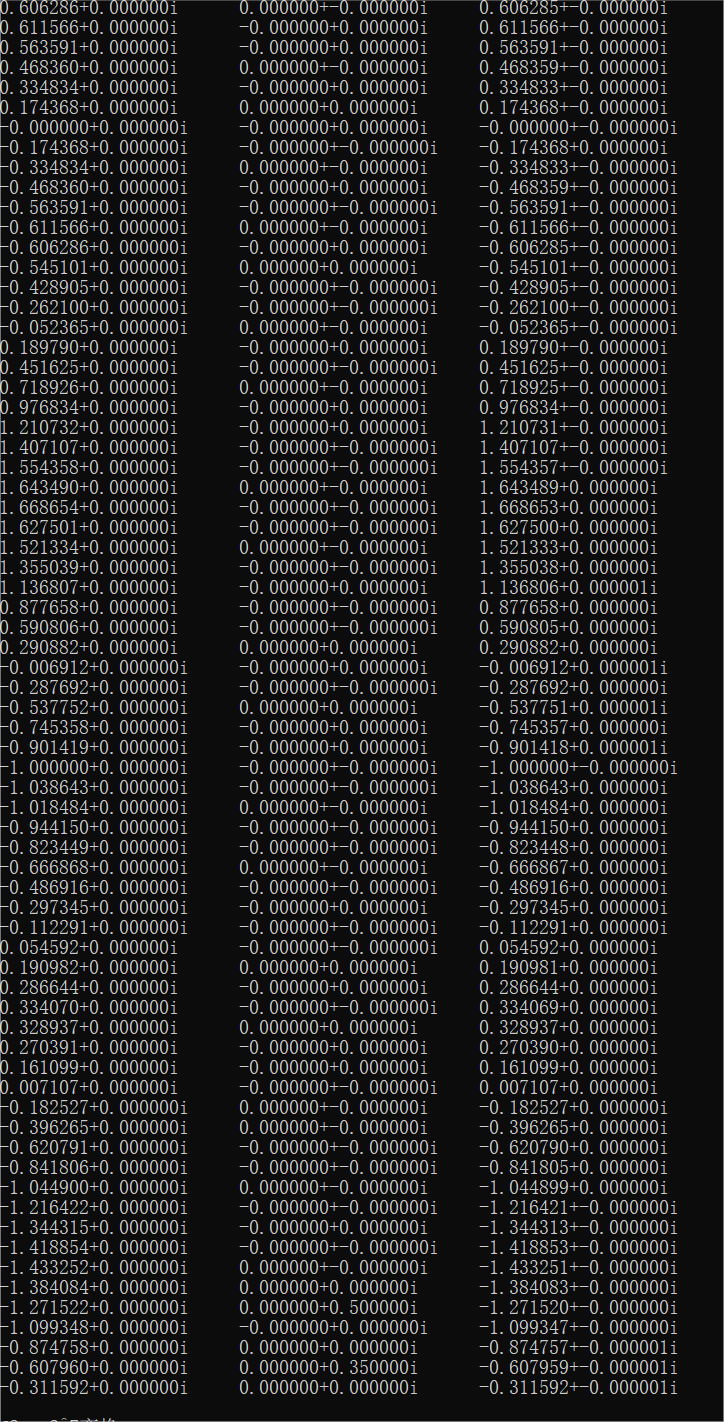
\includegraphics[scale=0.4]{f1_7(2)}
	\captionsetup{font={small},labelfont=bf}
	\caption{\heiti\zihao{-5}f1进行FFT结果(n=$ 2^7 $)2}
	
\end{figure}
	\begin{figure}[!h]
	
	\centering
	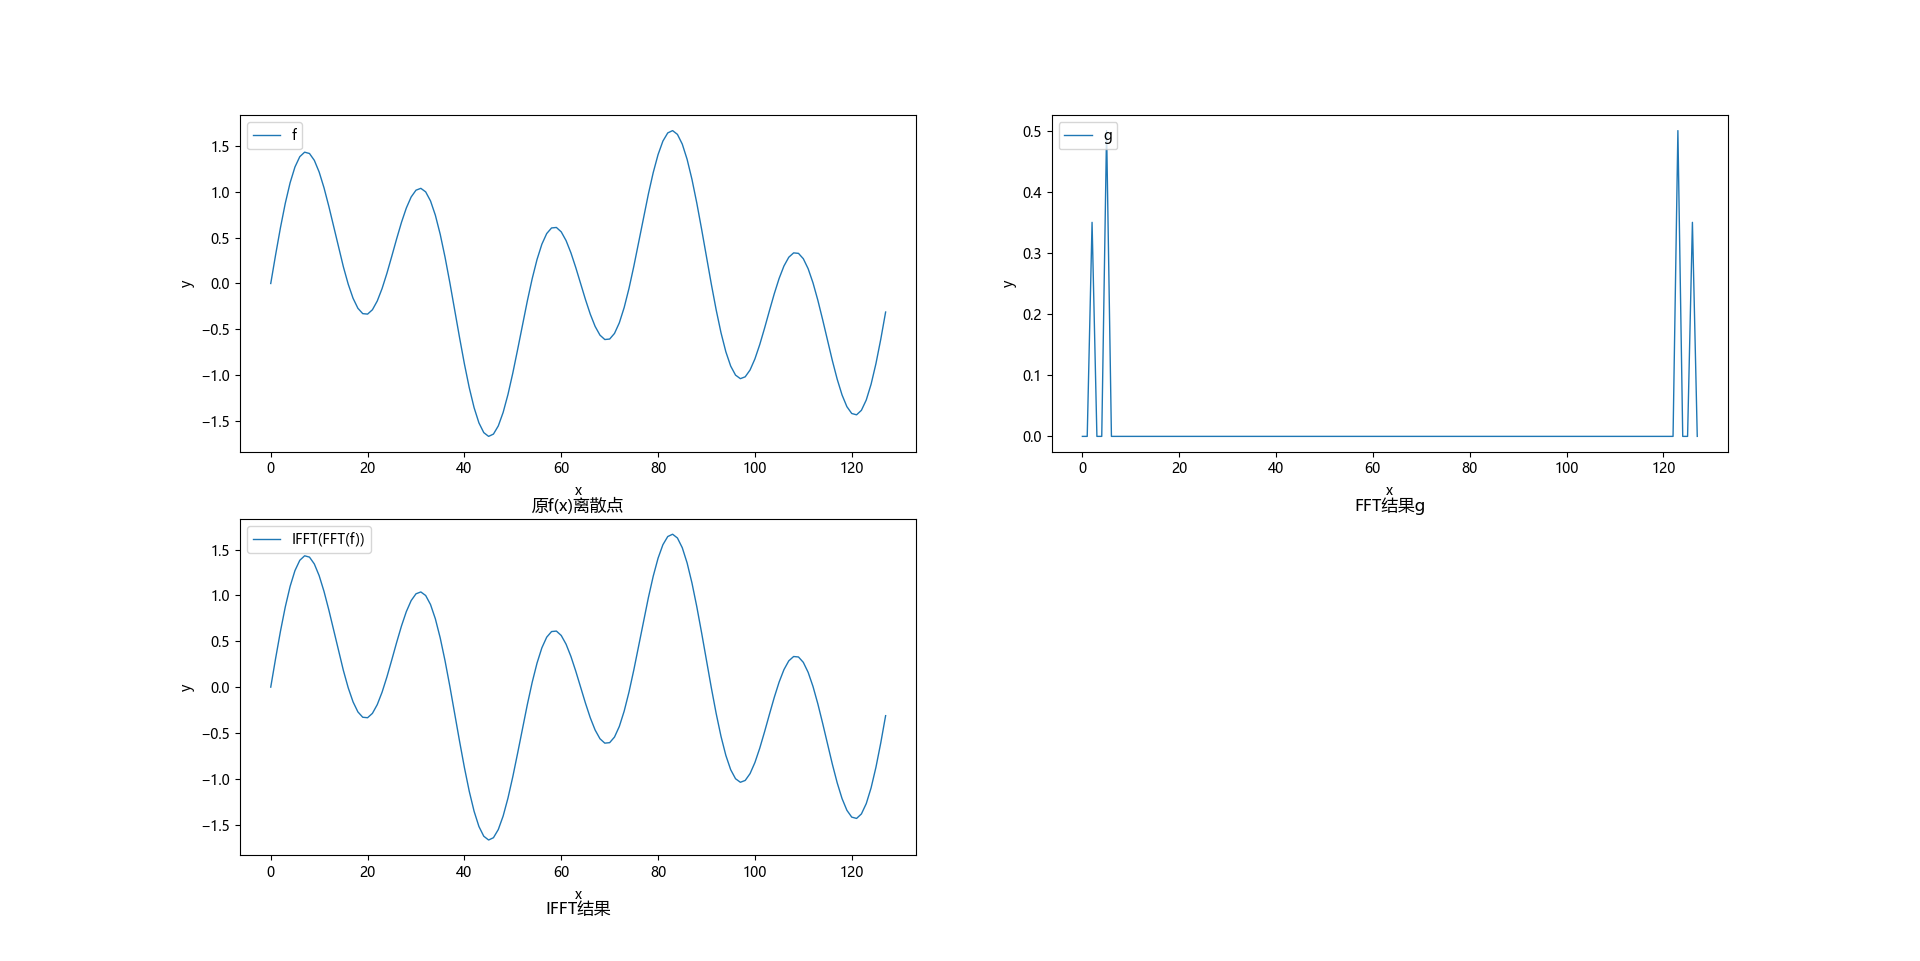
\includegraphics[scale=0.4]{f_1_7}
	\captionsetup{font={small},labelfont=bf}
	\caption{\heiti\zihao{-5}f1进行FFT结果(n=$ 2^7 $)}
	\label{fig:4}
\end{figure}
\begin{figure}[!h]
	
	\centering
	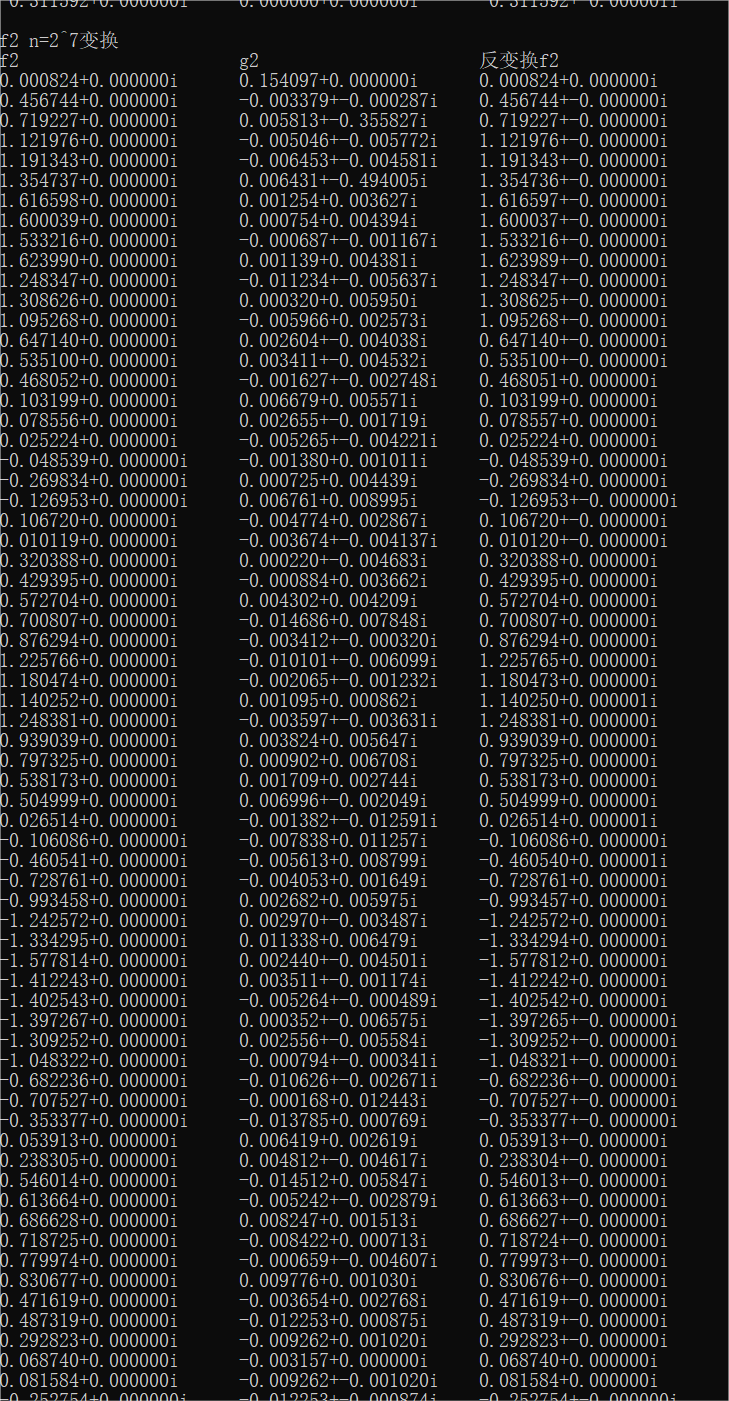
\includegraphics[scale=0.4]{f2}
	\captionsetup{font={small},labelfont=bf}
	\caption{\heiti\zihao{-5}f2进行FFT结果(n=$ 2^7 $)1}
	\label{fig:5}
\end{figure}
\begin{figure}[!h]
	
	\centering
	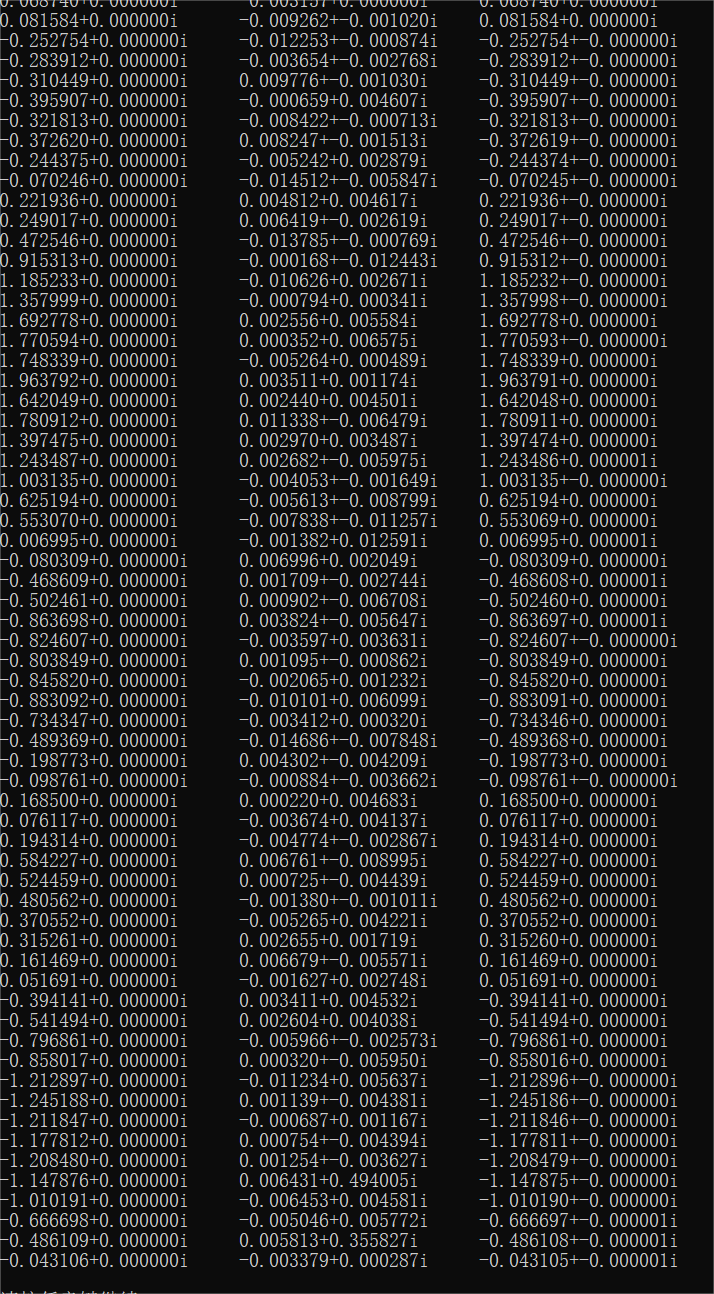
\includegraphics[scale=0.4]{f2(2)}
	\captionsetup{font={small},labelfont=bf}
	\caption{\heiti\zihao{-5}f2进行FFT结果(n=$ 2^7 $)2}
	
\end{figure}
	\begin{figure}[!h]
	
	\centering
	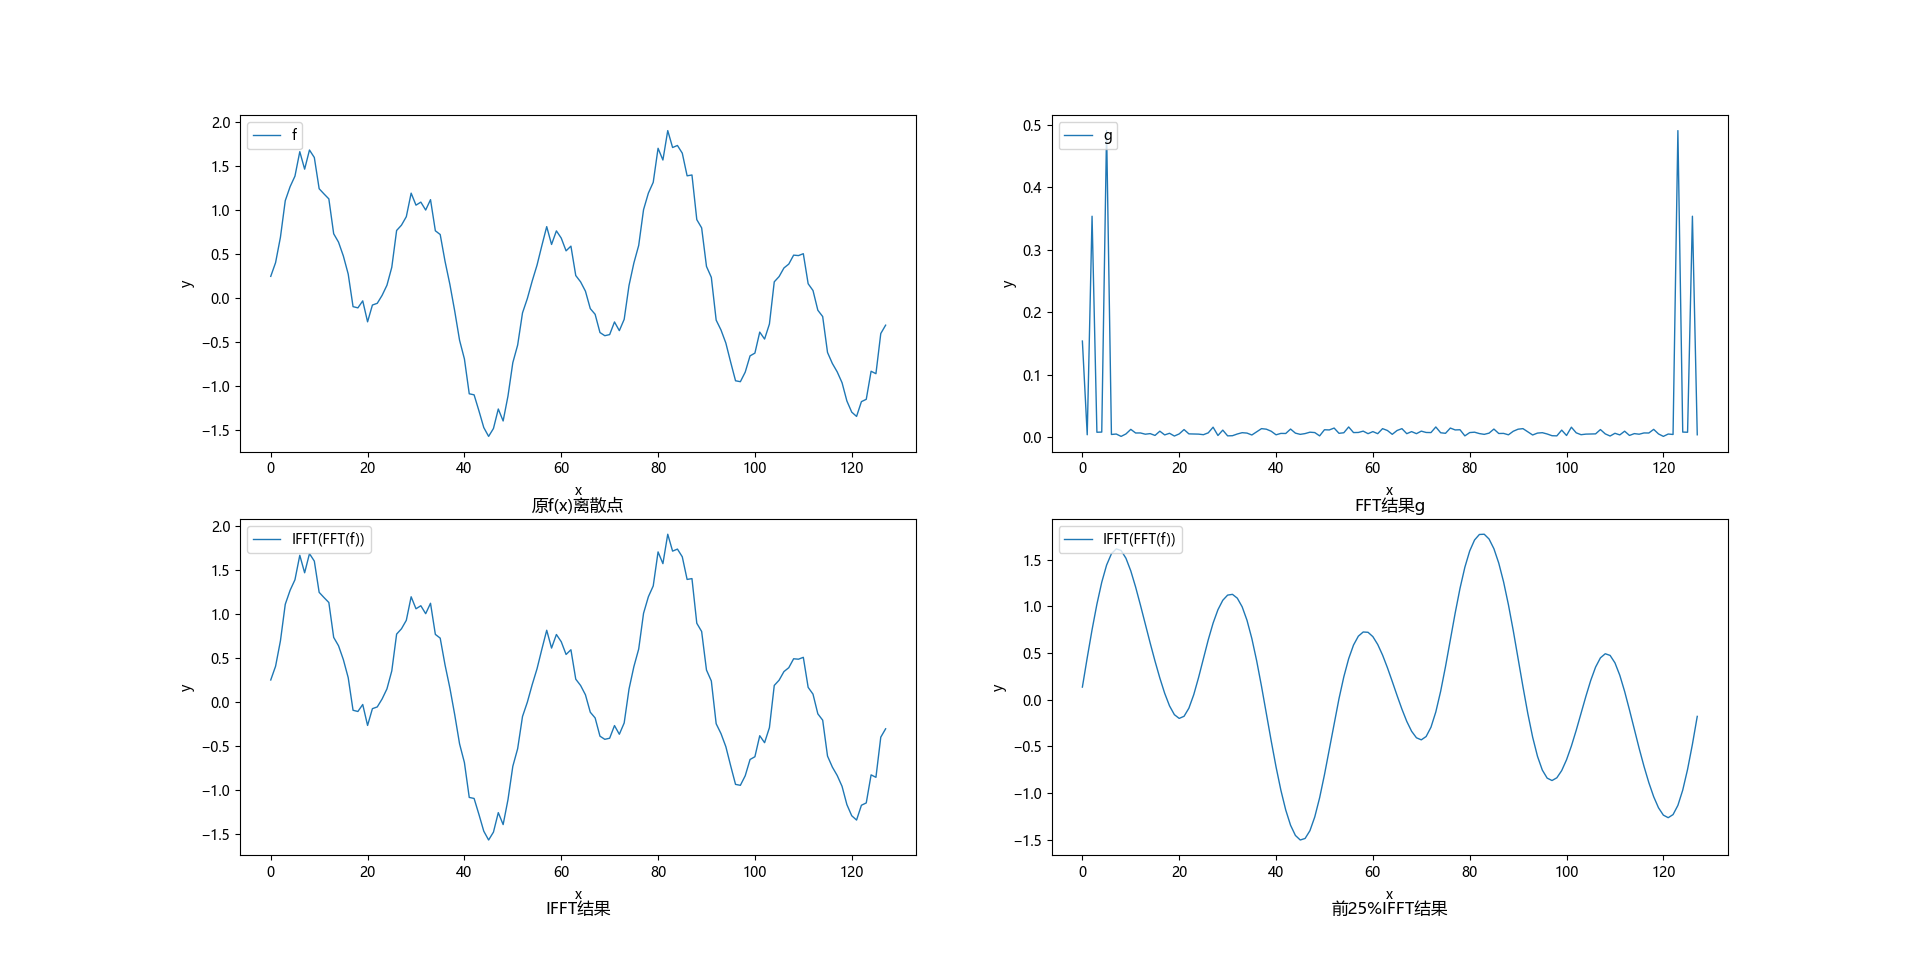
\includegraphics[scale=0.4]{f_2}
	\captionsetup{font={small},labelfont=bf}
	\caption{\heiti\zihao{-5}f2进行FFT结果(n=$ 2^7 $)}
	\label{fig:6}
\end{figure}

\end{document}